\begin{frame}{Motivation \& Preliminaries}

\onslide<1->{
\textbf{Reactive} stochastic project scheduling: S-RCPSP
\begin{itemize}
 	\item stochastic durations $\x{D}=(D_1, \ldots, D_n)$ with known $\mathbb{P}[D_i = t]$
 	\item solution = \sout{fixed schedule} scheduling policy $\Pi$
  	\item find $\Pi$ that minimizes $\mathbb{E}[\max_{i=1,\ldots,n} (S_i(\Pi,\x{D}) + D_i)]$
  	\item RCPSP generalization (at least as hard)
\end{itemize}

\medskip
}

\onslide<2->{
	Various classes of $\Pi$
 	\begin{itemize}
		\item list-based policies,  earliest-start policies, etc.  (M{\"o}hring et al. 1984,1985)
		\item exact procedures (Stork 2000)
		\item meta-heuristics (e.g. Ballest{\'\i}n 2007, Ashtiani et al. (2011))
	\end{itemize}
}

\end{frame}

\begin{frame}{Motivation \& Preliminaries}

Example S-RCPSP \& solution
\medskip
\begin{center}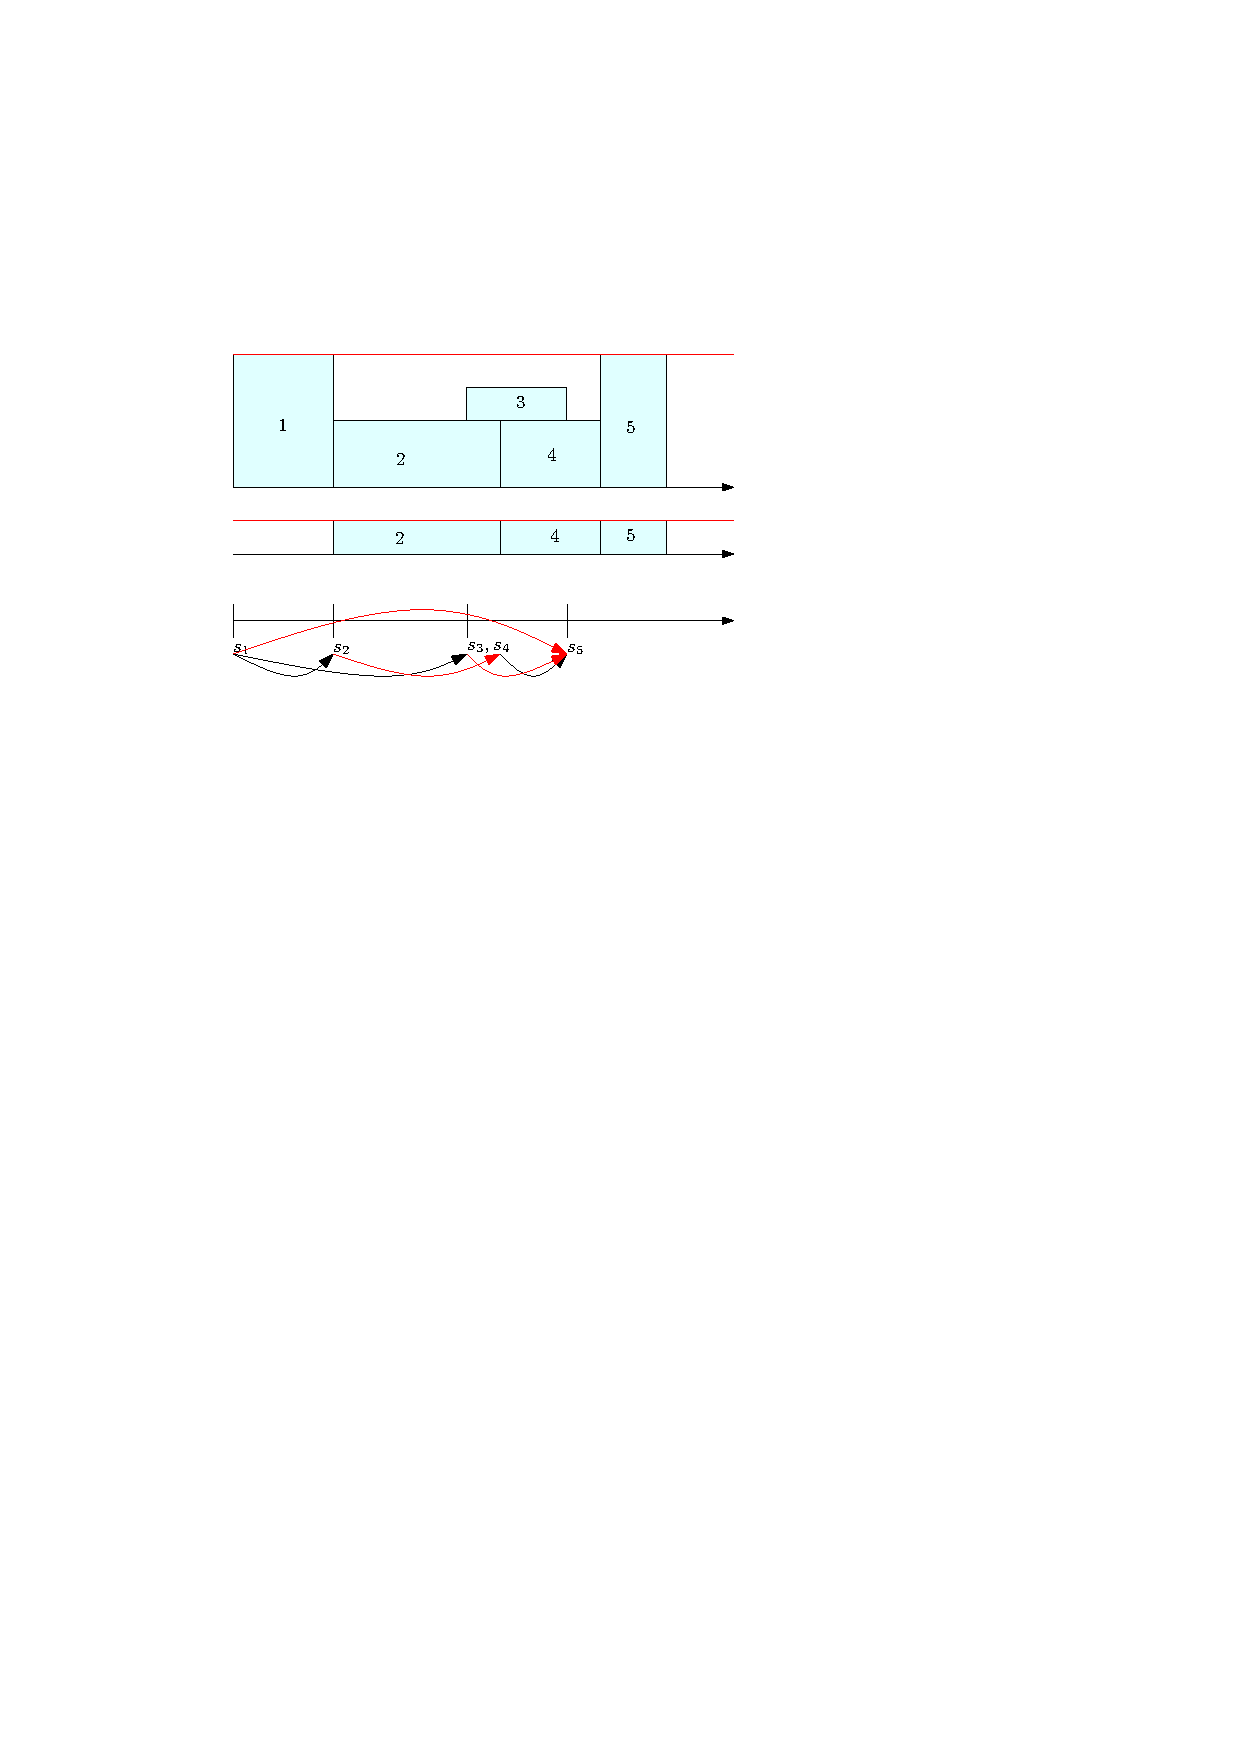
\includegraphics[width=0.7\textwidth]{fig-s1c}\end{center}
 
\onslide<2->{
	\medskip
	Disadvantage: no fixed-time schedule at all
}

\end{frame}

